\section{Hardware}

\subsection{Introducci\'on}
\label{Hintro}
Para nosotros, un robot recolector de residuos deb\'ia contar con caracter\'isticas que permitieran el sensado de un entorno f\'isico y din\'amico,
actuar seg\'un sus prop\'ositos y le proveyeran del mayor nivel de autonom\'ia energ\'etica y de interacci\'on humana posible.

Deb\'ia tener capacidades para reconocer distintos objetos en su campo de visi\'on y puder discernir entre la basura para recogerla y un
obst\'aculo para evitarlo.

Deb\'ia poder desplazarse y tener informaci\'on de su posici\'on respecto a la base para mantener a la bater\'ia recargada y
el recipiente interno disponible para nuevos res\'iduos. Tambi\'en deber\'ia poder seguir una l\'inea para dirigirse a la base o recalibrar
su posici\'on actual.

Seg\'un las especificaciones dadas, tuvimos en cuenta varias posibles implementaciones que explicamos y analizamos en la secci\'on \ref{HposiblesDisenos}.
Detallamos los distintos dispositivos de sensado, modos de locomoci\'on y actuadores que tuvimos en cuenta, sus caracter\'isticas principales y por qu\'e
los elegimos para la construcci\'on del robot.

En las secciones \ref{Hactuadores} y \ref{Hsensores} vemos, respectivamente, los actuadores y sensores que utilizamos finalmente para el armado
f\'isico del robot.
En la secci\'on \ref{Hcomm} analizamos cuestiones con respecto a la comunicaci\'on interna entre los distintos dispositivos.
En la secci\'on \ref{Harmado} explicamos aspectos de contrucci\'on, desde el dise\~no y armado de las placas controladoras hasta la
construcci\'on del primer prototipo del robot.

\subsection{Posibles dise\~nos e implementaci\'on}
\label{HposiblesDisenos}

Evaluamos distintos factores para la elecci\'on de cada dispositivo o m\'odulo presente en el robot. Desde la forma de desplazamiento hasta  el
m\'etodo de sensado, pasando por el controlador, captura de im\'agenes y m\'etodo de recolecci\'on de residuos. Estos son los factores que explicamos y
detallamos en este apartado.

\subsubsection{Locomoci\'on}

Por tratarse de un robot movil, la locomoci\'on fue un factor importante que tuvimos que resolver. En un principio la forma en que el robot iba a desplazarse,
si iba a ser mediante ruedas, orugas o patas. En segundo t\'ermino, requer\'iamos poder determinar y asegurar la velocidad a la cual se desplazaba,
saber la cantidad y sentido del desplazamiento y conocer su consumo.

La coordinaci\'on de las patas y el equilibrio del cuerpo implicaba una complejidad que escapaba el alcance del proyecto. El uso de orugas era una
excelente opci\'on como base para soporte del peso y prove\'ia buen equilibrio, pero la fricci\'on de las mismas generaba una posible falta de
precisi\'on que nos pod\'ia traer problemas para la detecci\'on de la cantidad de giro o desplazamiento y por ende, una incorrecta localizaci\'on en
el terreno. El uso de dos ruedas de tracci\'on y con al menos una tercer rueda de tipo castor para proveer equilibrio fue nuestra elecci\'on.
En la secci\'on \ref{Hactuadores} explicamos detalladamente la elecci\'on de los actuadores para esta y otras tareas.

\subsubsection{Sensado}

El sensado del ambiente englobaba varios puntos que deb\'iamos tener en cuenta a la hora de elegir la cantidad, forma, rango, m\'etodo y costo
de los sensores. En principio los requerimientos eran claros, necesitabamos poder detectar objetos en el ambiente, evitar obst\'aculos y realizar
mediciones internas al robot, como eran el nivel de bater\'ia, consumos y posici\'on de los motores.

La captura de im\'agenes deb\'ia ser realizada por medio de una c\'amara de video o webcam. Esta prove\'ia de la principal fuente de datos para
el proceso de reconocimiento de residuos explicado en el documento. Las distintas caracter\'isticas de la c\'amara como su resoluci\'on, refresco,
nivel de ruido, mejoras de la im\'agen y su velocidad de respuesta nos determinar\'ian la elecci\'on de la misma.

La detecci\'on de obst\'aculos implicaba otras caracter\'istcas de sensores. Principalmente de necesitabamos sensores de distancia con la apertura
necesaria para cubrir lo mejor posible, el per\'imetro del robot, otorgando un rango de detecci\'on lo suficientemente olgado que permitiera una adecuada
velocidad de respuesta al controlador principal para reacci\'onar y poder evitar objetos desconocidos o marcados como obst\'aculos.

Entre los distintos tipos de sensores de distancia estaban los de ultrasonido, tel\'emetros infrarrojos y scanners l\'aser. Los sensores de distancia
por ultrasonido tienen un rango aproximado entre 2 cent\'imetros y 4 metros en la zona de detecci\'on y un \'angulo de apertura variable seg\'un la
distancia al objetivo. El tiempo de espera que se debe tener entre disparo y disparo del sensor por posibles rebotes del pulso de sonido es
relativamente elevado, lo que no lo hace el m\'as adecuado para la colocaci\'on a lo largo del per\'imetro del robot. En contraparte los tel\'emetros
infrarrojos no poseen esta limitaci\'on debido a que la velocidad de la luz es superior a la del sonido. Pero los rangos efectivos de detecci\'on
de objetos no cubrian completamente nuestras necesidades.

Debido a las caracter\'isticas de los sensores decidimos combinarlos para aprovechar los beneficios de cada uno de ellos y suplir las falencias
de un tipo con otro el tipo. Un anillo de 8 tel\'emetros distribuidos de forma tal que haya una mayor resoluci\'on en la zona frontal del robot
contra la zona trasera y lateral y un \'unico sensor de distancia por ultrasonido al frente para captar objetos a mayor distancia.

El uso de un scanner l\'aser hubiera sido ideal para un an\'alisis topogr\'afico del terreno pero no era el caso y el elevado costo de los mismos los
dej\'o fuera de escala para el proyecto.

La detecci\'on de una l\'inea en el piso la resolvimos mediante el uso de sensores opticos reflectivos apuntando hacia el piso de manera tal que
permitieran diferenciar entre distintos niveles de reflexi\'on y por ende, diferenciar una l\'inea del piso.

Las caracter\'isticas de los sensores elegidos se explican con m\'as detalles en la secci\'on \ref{Hsensores}.

\subsubsection{Controlador}

Teniamos especificaciones que nos generaban la necesidad de ejercer control sobre los distitnos dispositivos presentes en el robot, ya sea para
obtener la informaci\'on que proveen, configurar los sensores, para controlar la velocidad de las ruedas o mismo para comunicar las distintas partes.
No exist\'ia una \'unica forma para realizar esto.

Experiencias previas nos daban la idea de tener un \'unico controlador que mantuviera el control de cada dispositivo. Esto generaba grandes exigencias de hardware y
una alta complejidad de dise\~no a nivel software para mantener en funcionamiento cada dispositivo. Otra opci\'on era la existencia de peque\~nos
controladores distribuidos con menor capacidad de procesamiento, destinados a pocas o una \'unica tarea, de dise\~no simple y con una menor complejidad
a nivel software. Esta soluci\'on combinada con una buena modularizaci\'on y una comunicaci\'on acorde, generaba a nuestra visi\'on y seg\'un
nuestras necesidades, la mejor opci\'on y por ende, fue la elegida.
En la secci\'on \ref{Hcomm} se explica todo lo referente a la comunicaci\'on entre m\'odulos, en la secci\'on \ref{Hmicro} explicamos detalladamente
la elecci\'on de los controladores y en la secci\'on \ref{Harmado} el dise\~no y construcci\'on de las placas.

Como la captura de im\'agenes se realizar\'ia por medio de una c\'amara de video, webcam o alg\'un otro tipo de c\'amara integrada y todo el
procesamiento de im\'agenes requiere grandes capacidades de c\'alculo, se resolvi\'o por simplicidad el uso de una computadora preferentemente de
arquitectura x86 para facilitar la compatibilidad a nivel software y por ende la inclinaci\'on al uso de una webcam con puerto USB como principal
dispositivo de captura de im\'agenes.
Por su bater\'ia propia de gran capacidad, facilidad de uso, disponibilidad de sistema operativo y entorno de desarrollo, costos y soporte a nivel
repuestos, se eligi\'o una netbook como controlador principal del robot.

\subsubsection{Recolecci\'on}

La necesidad de recolecci\'on de basura del robot nos suger\'ia la existencia de un mecanismo que permitiera tomar objetos y llevarlos al recipiente
interior para la futura descarga. Entre las opciones que tuvimos en cuenta la existencia de un brazo mec\'anico con los suficientes grados de
libertad para realizar la tarea, idea que rechazamos por las dificultades de control y construcci\'on que s\'olo el brazo generaban. Otra opci\'on fue
un mecanismo de aspirado de los residuos hacia el interior, pero esta soluci\'on no nos permit\'ia diferenciar entre lo que se recolectaba, juntar
colillas de cigarrillos, vasos o botellas y generaba gran consumo de energ\'ia. Finalmente elegimos una soluci\'on que constaba de una pala que se
extiend\'ia, recog\'ia y contra\'ia para dejar los residuos en el recipiente. Aunque por falta de tiempo el mecanismo no fue implementado para la
presentaci\'on y armado f\'isico del prototipo.

\subsection{Actuadores}
\label{Hactuadores}

	Los actuadores son la principal forma en que el robot puede interactuar en forma activa con el medio que lo rodea. Hay distintas partes que necesitan
	este tipo de dispositivos, la tracci\'on principal de las ruedas, el movimiento del m\'odulo de recolecci\'on y de otras partes como podr\'ian ser una
	c\'amara con paneo y giro o un senor de ultrasonido colocado en la parte superior haciendo las veces de radar.
	Estas cuestiones se analizan en este apartado.

\subsubsection{Motores principales}
\label{HmotoresP}

	Eran parte de los requerimientos el poder garantizar una velocidad determinada en los motores para la tracci\'on de las ruedas, poder mantener
	un control de la cantidad de movimiento independiente en cada rueda, conocer las vueltas dadas por cada una de las ruedas y era deseable
	la posibilidaded de poder especificar la cantidad de vueltas a realizar para luego detenerse sin intervenci\'on del controlador principal.
	
	Para este trabajo elegimos motores de corriente cont\'inua ya que pod\'iamos satisfacer todas las necesidades con simplicidad para su control. Los motores
	elegidos son de la marca Ignis \footnote{http://www.ignis.com.ar} modelo \emph{MR-2FA} que esta provisto de una caja reductora con caracter\'isticas
	expresadas en la tabla \ref{HTmotorDC}, tambi\'en poseen un encoder de $4$ estados por vuelta en el eje del motor y un sensor de revoluci\'on completa a la salida de
	la caja reductora. En la secci\'on \ref{HSencodersConsumo} explicamos detalladamente el funcionamiento de los encoders y medici\'on del consumo del motor.
	
	\begin{table}
		\begin{center}
			\begin{tabular}{|l|c|c|c|c|}
				\hline
				Caracter\'istica & Unidad & M\'inimo & Nominal & M\'aximo \\
				\hline
				Tensi\'on & V & 8 & 9 & 12 \\
				Corriente & A & 0.6 & 1.2 & 2.4 \\
				Velocidad & RPM & 1 & 60 & 60 \\
				Aceleraci\'on & $1/s^{2}$ & 0.1 & 0.1 & 0.5 \\
				Torque & kgf*cm & 0 & 1.2 & 6.4 \\
				\hline
			\end{tabular}
		\end{center}
		\caption{Caracter\'isticas del motor Ignis MR-2FA.}
		\label{HTmotorDC}
	\end{table}
	
	En la secci\'on \ref{HAPmotorDC} explicamos detalladamente la construcci\'on y principios de funcionamiento de la placa controladora para estos motores.

\subsubsection{Actuadores de uso m\'ultiple}
\label{HactuadoresVarios}

Otros tipos de actuadores tambi\'en eran necesarios para poder realizar la tarea de la recolecci\'on de residuos, ya sea para accionar el mecanismo
que juntar\'ia la basura o inclinar el robot para una mejor recolecci\'on.
Para estas tareas los servo motores nos parecieron ideales por su facilidad de uso y control, pero el torque que pose\'ian no era suficiente para todas las tareas.
En consecuencia luego de buscar otras alternativas, elegimos nuevamente el uso de motores de cont\'inua con un mecanismo con un tornillo sin fin para aumentar el
torque final de los mismos. Nuevamente elegimos la combinaci\'on de ambas soluciones. En la secci\'on \ref{HAPservos} explicamos en detalle
el dise\~no de las placas controladoras de servos, aunque no fueron contruidas porque no se hab\'ia terminado el dise\~no del mecanismo de
recolecci\'on a la fecha de la construcci\'on del prototipo. Para el control de los motores de cont\'inua podr\'ian utilizarse placas similares a las
explicadas en la secci\'on \ref{HAPmotorDC} con las modificaciones que requiera la aplicaci\'on.

\subsection{Sensores}
\label{Hsensores}

En este apartado explicamos detalladamente cada uno de los tipos de sensores que utilizamos para realizar tanto las mediciones externars como las
internas al al robot. Analizamos las ventajas de cada uno, los posibles problemas que pueden surgir y las soluciones a los mismos.
En la secci\'on \ref{HAPsensores} explicamos el dise\~no y construcci\'on de las placas que controlan todos los sensores del robot.

\subsubsection{Sensores de distancia por ultrasonido}
\label{HSultrasonido}

El sensor de distancia por ultrasonido que elegimos es el modelo \emph{SRF05} de la marca Devantech Ltd \footnote{http://www.robot-electronics.co.uk/}.
Es la versi\'on mejorada del modelo \emph{SRF04}, la cual aumenta el rango de detecci\'on y mejora el modo de control y lectura de los datos, permitiendo
hacerlo mediante un \'unico pin.

El principio de funcionamiento es relativamente sencillo, mediante un peque\~no pulso en el pin de \emph{TRIGGER}, se genera un tren de $8$ pulsos
ultras\'onicos y luego se espera como respuesta, el mismo tren de pulsos que deber\'ia haber rebotado contra el objetivo. En base a la diferencia de tiempo
entre la emisi\'on del tren de pulsos y la respuesta, se calcula la distancia a la que se encuentra el objetivo. La distancia es codificada en el ancho
de un pulso que var\'ia de $100\mu s$ a $25 ms$. Si dentro del rango de detecci\'on no se encuentra ning\'un objeto, el pulso tendr\'a un ancho
de $30$ milisengundos.

En la tabla \ref{HTultrasonido} detallamos las caracter\'sticas del sensor \emph{SRF05} y en la figura \ref{HFultrasonido} mostramos el haz ultras\'onico
del sensor.

\begin{table}[ht]
	\begin{center}
		\begin{tabular}{|l|c|c|}
			\hline
			Caracter\'istica & Unidad & Valor\\
			\hline
			Tensi\'on de alimentaci\'on & $V$ & 5 \\
			Frecuencia de trabajo & $KHz$ & 40 \\
			Rango m\'aximo & $cm$ & 400 \\
			Rango m\'inimo & $cm$ & 1.7 \\
			Duración m\'inima del pulso de disparo & $\mu s$ & 10 \\
			Duración del pulso eco de salida & $\mu s$& 100 - 25000 \\
			Tiempo m\'inimo de espera entre mediciones & $m s$ & 20 \\
			\hline
		\end{tabular}
	\end{center}
	\caption{Caracter\'isticas del sensor de distancia por ultrasonido SRF05.}
	\label{HTultrasonido}
\end{table}

\begin{figure}[ht]
	\centering
	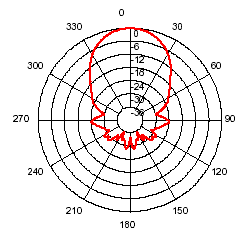
\includegraphics[scale=0.5]{us-beam.png}
	\caption{Haz ultras\'onico del sensor de distancia por ultrasonido SRF05.}
	\label{HFultrasonido}
\end{figure}

\subsubsection{Tel\'emetros infrarrojos}
\label{HStelemetros}

Los tel\'emetros por infrarrojo que elegimos son el modelo \emph{GP2D120} de Sharp \footnote{http://sharp-world.com/products/device}.

El principio de funcionamiento de este tipo de sensores es mediante un haz de luz infrarroja que es emitido hacia el objetivo, el cual
es reflejado y captado a traves de un lente por un sensor de posici\'on relativa en el interior del sensor. En base a esta medici\'on
se calcula la distancia entre el sensor y el objeto reflectivo que se encuentra frente a \'el. La salida es anal\'ogica para este
modelo espec\'ifico.

\begin{table}[ht]
	\begin{center}
		\begin{tabular}{|l|c|c|}
			\hline
			Caracter\'istica & Unidad & Valor\\
			\hline
			Rango m\'aximo & $cm$ & 30 \\
			Rango m\'inimo & $cm$ & 4 \\
			Tensi\'on para la m\'axima distancia & $V$ & 1.95 \\
			Tensi\'on para la m\'inima distancia & $V$ & 2.55 \\
			Tensi\'on de alimentaci\'on & $V$ & 5 \\
			Consumo m\'aximo & $mA$ & 50 \\
			\hline
		\end{tabular}
	\end{center}
	\caption{Caracter\'isticas del sensor de distancia por ultrasonido SRF05.}
	\label{HTtel}
\end{table}

En la tabla \ref{HTtel} detallamos los valores caracter\'isticos del modelo. En la figura \ref{HFteldistancia} mostramos la tabla de
conversi\'on entre voltaje de salida y distancia al objeto, y en la figura \ref{HFtelapertura} mostramos el \'angulo de apertura de
la zona de detecci\'on seg\'un la distancia al objetivo.

\begin{figure}[ht]
	\centering
	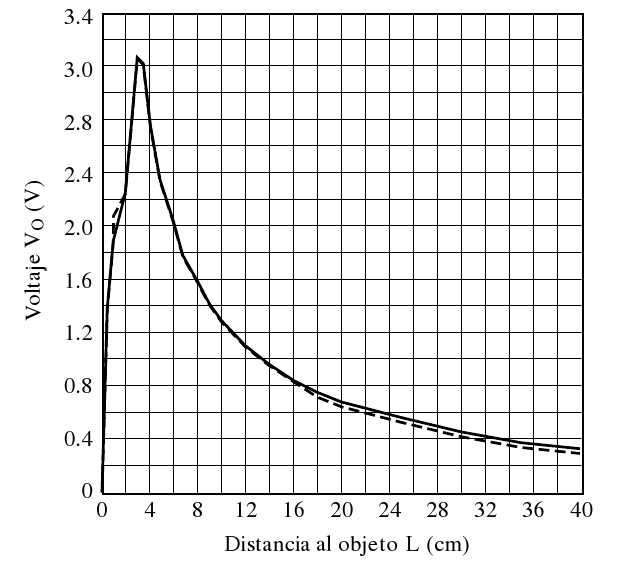
\includegraphics[scale=0.35]{tel-VxL.png}
	\caption{Voltaje de salida seg\'un la distancia al objeto del tel\'emetro GP2D120.}
	\label{HFteldistancia}
\end{figure}


\begin{figure}[ht]
	\centering
	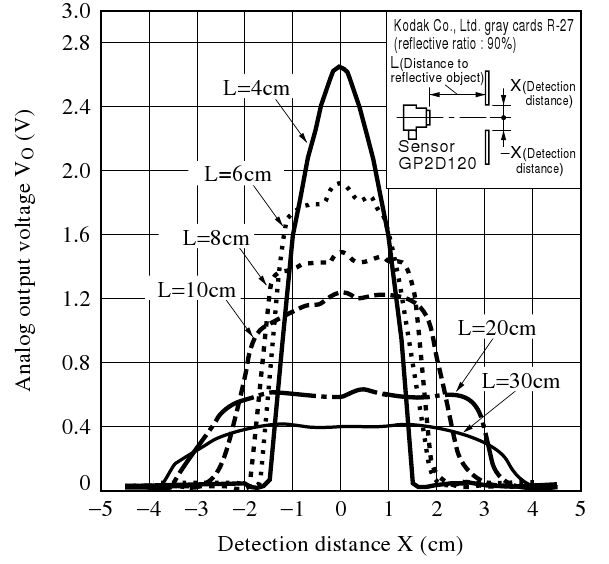
\includegraphics[scale=0.35]{tel-VxX.png}
	\caption{\'Angulo de apertura seg\'un la distancia del tel\'emetro GP2D120.}
	\label{HFtelapertura}
\end{figure}

\subsubsection{Sensores reflectivos de piso}
\label{Hpiso}

Los sensores que elegimos para sensar la l\'inea reflectiva en el piso son el modelo \emph{CNY70} de la marca Vishay Semiconductor
\footnote{http://www.vishay.com/}.

Son sensores opticos reflectivos que captan el nivel de luz emitida por el mismo sensor y reflejada sobre la superf\'icie a sensar
como se muestra en la figura \ref{HFpiso}. En la figura \ref{HFpisoID} mostramos la corriente que circula por el colector del
fototransistor en base a la distancia al objeto medido.

El rango efectivo de sensado ronda los $3 mm$ de distancia, aunque con un incremento en la corriente que circula por el emisor de luz
se puede llegar a una distancia mayor que permita un uso m\'as acorde al proyecto.

\begin{figure}[ht]
	\centering
	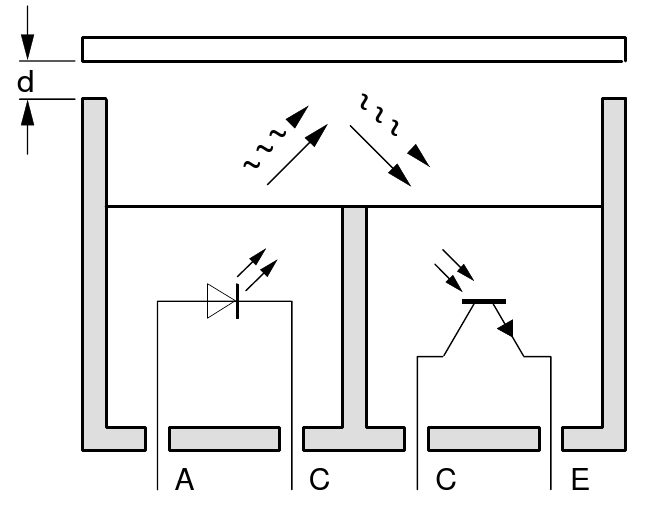
\includegraphics[scale=0.15]{piso.png}
	\caption{Principio de funcionamiento del sensor reflectivo CNY70.}
	\label{HFpiso}
\end{figure}


\begin{figure}[ht]
	\centering
	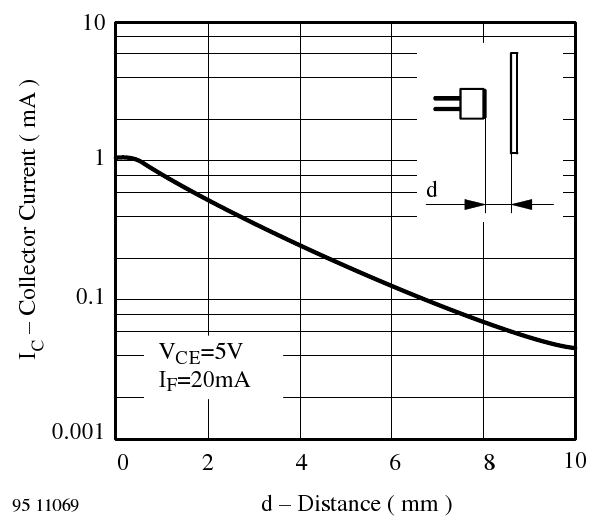
\includegraphics[scale=0.35]{piso-IxD.png}
	\caption{Corriente en el colector seg\'un la distancia del sensor CNY70.}
	\label{HFpisoID}
\end{figure}

\subsubsection{Sensado de nivel de bateria}
\label{HSnivelBateria}

El sensado del nivel de tensi\'on en la bater\'ia lo hacemos mediante un divisor de tensi\'on entre los polos de la bater\'ia.
La salida es sensada de igual forma que los otros sensores. En la secci\'on \ref{HAPsensores} explicamos mas en detalle la conexi\'on.
En la figura \ref{HFbateria} mostramos el diagrama del divisor de tensi\'on.

\begin{figure}[ht]
	\centering
	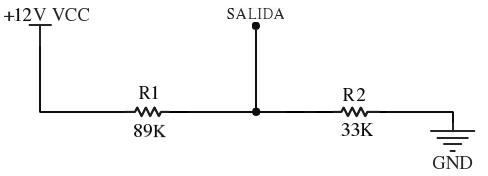
\includegraphics[scale=0.35]{bateria.png}
	\caption{Divisor de tensi\'on para el sensado de la bater\'ia.}
	\label{HFbateria}
\end{figure}

En la tabla \ref{HTdivT} mostramos las posibles tensiones en la bater\'ia y la tensi\'on de salida en el divisor. Tambi\'en incluimos el
valor aproximado para un conversor anal\'ogico digital con tensi\'on de referencia a $5V$ que leer\'ia la salida del divisor. El rango de
voltajes que analizamos tiene en cuenta la posibilidad de efectuar mediciones durante la carga de la bater\'ia y sabiendo que con una
tensi\'on menor a $5 V$ la l\'ogica del prototipo construido comenzar\'ia a fallar.

\begin{table}[ht]
	\begin{center}
		\begin{tabular}{|c|c|c|c|}
			\hline
			Bater\'ia ($V$) & Salida ($V$) & Valor en el ADC ($5V$) \\
			\hline
			16 & 4.327 & 886 \\
			15 & 4.057 & 831 \\
			14 & 3.786 & 776 \\
			13 & 3.516 & 720 \\
			12 & 3.245 & 665 \\
			11 & 2.975 & 609 \\
			10 & 2.704 & 554 \\
			 9 & 2.434 & 499 \\
			 8 & 2.163 & 443 \\
			 7 & 1.893 & 388 \\
			 6 & 1.623 & 332 \\
			 5 & 1.352 & 277 \\
			\hline
		\end{tabular}
	\end{center}
	\caption{Tensi\'on de la bater\'ia y la tensi\'on de salida en el divisor.}
	\label{HTdivT}
\end{table}

\subsubsection{Encoders y consumo de los motores}
\label{HSencodersConsumo}

Los motores \emph{MR-2FA} tienen encoders de cuadratura conectados al eje, previo a la caja reductora. Estos encoders son
de tipo fotoel\'ectricos, estan dispuestos a $135^{\circ}$ uno del otro y marcan $4$ estados por cada vuelta del motor.
Los utilizamos para medir y controlar la velocidad de los motores tomando la cantidad de vueltas por escala de tiempo.

El consumo de los motores, lo medimos leyendo el pin de sensado que se encuentra en el puente H que alimenta al motor, como
explicamos en la secci\'on \ref{HAPmotorDC}.

\subsection{Comunicaci\'on entre m\'odulos}
\label{Hcomm}

La comunicaci\'on entre los distintos componentes del robot es imprescindible para su correcto funcionamiento. Todos los comandos
originados en el controlador principal viajan por este este medio de comuncaciones y debemos asegurarnos que llegan de forma correcta
y a tiempo para realizar las distintas tareas que se necesiten.

En este apartado explicamos en detalle las decisiones que tomamos para crear una comunicaci\'on acorde a nuestras necesidades.

\subsubsection{Conectividad entre los m\'odulos de control}
\label{HCconectividad}

Para establecer el canal de comunicaciones decidimos emplear una configuraci\'on basada en el m\'etodo \emph{Daisy-Chain}
\footnote{Patente US20090316836A1} entre las distintas placas controladoras creando un anillo donde cada nodo de la cadena se
comunica con su vecino retransmitiendo cada paquete hacia adenlante hasta su destinatario como mostramos en la figura
\ref{daisychain_diagram}.

\begin{figure}[ht]
	\centering
	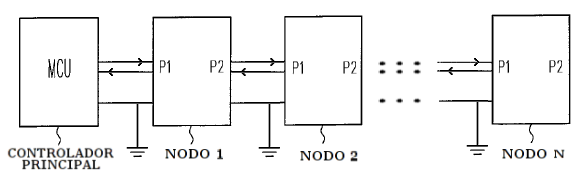
\includegraphics[scale=.40]{daisychain_diagram.png}
	\caption{Diagrama general del m\'etodo daisy chain}
	\label{daisychain_diagram}
\end{figure}

La configuraci\'on que elegimos para realizar la comunicaci\'on fue una velocidad de $115200$ baudios, $8$ bits, con $1$ bit de parada,
sin bit de paridad y sin control de flujo. Logramos una gran velocidad de respuesta a los comandos de esta forma.

\subsubsection{Protocolo de comunicaci\'on}
\label{HCprotocolo}

El protocolo de comuncaci\'on est\'a formado por paquetes que tienen un formato espec\'ifico y representan un pedido de informaci\'on o
comando que debe ser ejecutado en el destino. 

El paquete consta de un header com\'un con datos que identifican el emisor y receptor del paquete, el comando a enviar y posibles datos
extras que sean requeridos. En el cuadro \ref{Hformato_paquete_tabla} se muestra la estructura interna de un paquete t\'ipico.

\begin{table}[ht]
	\begin{center}
		\begin{tabular}{|c|c|c|c|c|c|}
			\hline
			LARGO & DESTINO & ORIGEN & COMANDO & DATO & CRC \\
			\hline
		\end{tabular}
	\caption{Formato y header del paquete de datos}
	\label{Hformato_paquete_tabla}
	\end{center}
\end{table}

Todos los paquetes tienen una respuesta obligatoria de confirmaci\'on de recepci\'on. Cuando el paquete requiera una respuesta
con datos, la confirmaci\'on ir\'a acompa\~nada de la informaci\'on requerida.

El control de errores se realiza mediante el checksum calculado haciendo un \emph{XOR} con cada byte del contenido del paquete
y colocado en el campo \emph{CRC}. Cuando un paquete se encuentre con errores o est\'e mal formado, el destinarario deber\'ia
pedir la retrasmisi\'on. De igual forma, creamos un control adicional por medio una lista de paquetes no confirmados mantenida
por el controlador principal.

Creamos un grupo de identidicaci\'on para cada placa controladora y un n\'umero que identifica a distintas placas de un mismo
tipo. De esta forma cada placa tiene un c\'odigo \'unico dentro de la cadena de comunicaci\'on evitando as\'i errores en el
destinatario del mensaje.

El listado de grupos y comandos correspondientes a cada grupo de controladores se encuentra en el ap\'endice \ref{HAppProtocolo}.

\subsection{El microcontrolador}
\label{Hmicro}

El microcontrolador que elegimos para realizar las tareas de control, configucari\'on y comunicaci\'on a bajo nivel es el \emph{PIC16F88} de
Microchip \footnote{http://www.microchip.com/}. Cuenta con una memoria \emph{FLASH} para 4096 instrucciones de programa, una memoria
\emph{RAM} de 368 bytes y una memoria \emph{EEPROM} de 256 bytes. Tiene un set de instrucciones b\'asicas reducido, todas con el mismo
tiempo de ejecuci\'on. En este apartado nombramos algunos de los principales perif\'ericos incluidos en el microcontrolador y la utilidad
dentro del proyecto que encontramos para ellos. Utilizamos con un cristal externo de 20MHz como clock.

\begin{figure}[ht]
	\centering
	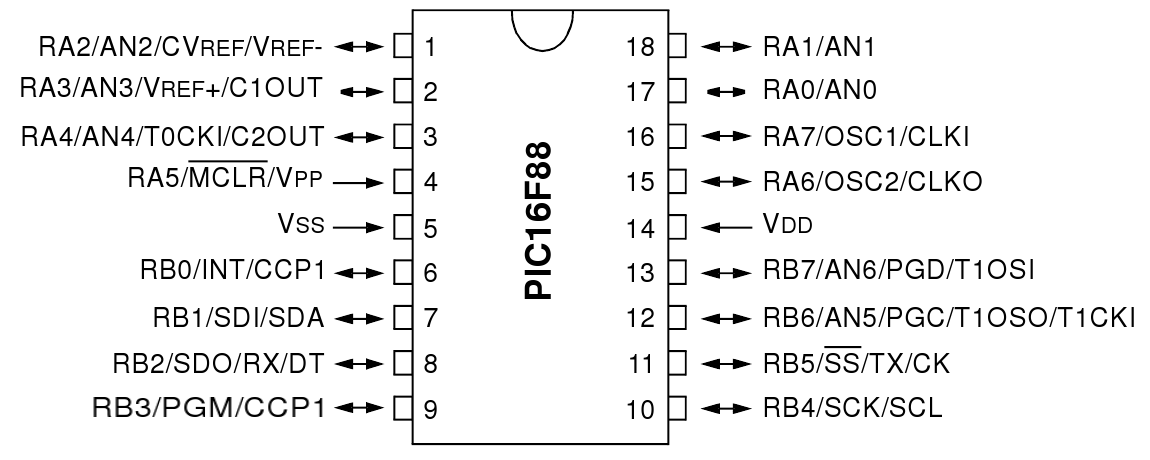
\includegraphics[scale=0.20]{pic16f88.png}
	\caption{Diagrama del microcontrolador PIC16F88.}
	\label{HFpic16f88}
\end{figure}

El microcontrolador tiene 2 puertos de 8 entradas y salidas cada uno de tipo TTL y CMOS.
Como mostramos en la figura \ref{HFpic16f88} cada pin se encuentra multiplexado con uno o m\'as perif\'ericos internos.

\subsubsection{AUSART}
\label{HMrs232}

Cuenta con un m\'odulo de UART para comunicaci\'ion sincr\'onica o asincr\'onica con un buffer por hardware de 3 bytes.

Este m\'odulo lo utilizamos para la implementaci\'on del daisy chain por RS-232 que comunica a todas las placas entre
ellas y a la controladora principal como explicamos en la secci\'on \ref{Hcomm}.

\subsubsection{Timers}
\label{timers}

Cuenta con 3 timers o contadores.

El \emph{TMR0} es de 8 bits y contiene un \emph{preescaler} de 8 bits, es usado como WDT.
Tambi\'en puede ser utilizado como contador externo por el pin \emph{RA4}.

El \emph{TMR1} es de 16 bits y contiene un \emph{preescaler} de 2 bits.
Puede ser utilizado como contador externo por el pin \emph{RB6} o con un cristal externo conectado a los pines \emph{RB6} y \emph{RB7}.

El \emph{TMR2} es de 8 bits, contiene un \emph{preescaler} de 2 bits y contiene un \emph{postscaler} de 4 bits.
Es de vital importancia para el m\'odulo de PWM por hardware.

Estos timers los utilizamos como base de tiempo o contadores en las placas controladoras como explicamos en las secciones \ref{HAPmotorDC},
\ref{HAPsensores} y \ref{HAPservos}.

\subsubsection{ADC}
\label{adc}

Cuenta con un conversor anal\'ogico digital de 8 o 10 bits multiplexado en 7 canales, 5 canales en el puerto A y 2 en el puerto B.
Es posible definir voltajes de referencia mediante ciertos pines o usar valores internos de referencia como \emph{Vcc} y \emph{GND}.

Lo utilizamos para realizar las mediciones sobre las salidas de los sensores de piso, los tel\'emetros infrarrojos, el nivel de tensi\'on en la bater\'ia
y para medir el consumo generado por los motores de cont\'inua.

\subsubsection{PWM}
\label{pwm}

Cuenta con un m\'odulo de generaci\'on de un PWM por hardware de 10 bits de resoluci\'on con el ciclo y per\'iodo configurable mediante el \emph{TMR2}.

Lo usamos para generar pulsos de ancho controlado para manejar la potencia que reciben los motores principales y en consecuencia, la velocidad de las ruedas.

\subsubsection{Otros}
\label{otros}

Para mayor informaci\'on respecto a los perif\'ericos o configuraci\'on del microcontrolador, recomiendamos revisar las hojas de datos en el sitio del fabricante.

\subsubsection{Programador}
\label{HMprogramador}

El programador que utilizamos es el modelo \emph{ICD2} de la empresa Microchip. El cual nos provee una interfaz tanto para la carga y descarga
de firmware al microcontrolador, sino que tambi\'en permite debuguear dicho c\'odigo.

La IDE de programaci\'on que usamos fue \emph{Microchip MPLAB} debido a su completa integraci\'on con el producto.

El lenguaje de programaci\'on fue \emph{C} y el compilador elegido \emph{CCS PCM V4.023}.

\subsection{Armado f\'isico del prototipo}
\label{Harmado}

\emph{armado fisico -> placas, ruedas, chasis, bateria, netbook}




*** NO TERMINADO ***




\subsubsection{Placa gen\'erica}
\label{HAPgenerica}

placa base - principio de funcionamiento, diseño y circuito a un apendice?
comunicacion, configuracion, modulo para la comunicacion, pines, conectores, switch




*** NO TERMINADO ***





\subsubsection{Placa controladora de motor de cont\'inua}
\label{HAPmotorDC}

En la placa controladora de los motores de tracci\'on principales, utilizamos el timer \emph{TMR0} como reloj para controlar la
velocidad de las ruedas. Configurado para que genere un interrupci\'on cada aproximadamente $6.25 ms$. El \emph{TMR1} lo utilizamos como
contador externo de las cuentas del encoder. Usando la base de tiempo generada por el \emph{TMR0}, conocemos con precisi\'on la velocidad
de las ruedas.


controladora de motorDC.
principio de funcionamiento.
configuracion x hardware, valores maximos y minimos que soporta.
diseño y circuito a un apendice?






*** NO TERMINADO ***



\subsubsection{Placa controladora de servo motores}
\label{HAPservos}

controladora de servos.
principio de funcionamiento.
configuracion x hardware, valores maximos y minimos que soporta.
diseño y circuito a un apendice?




*** NO TERMINADO ***





\subsubsection{Placa controladora de sensores}
\label{HAPsensores}

En la placa controladora de los sensores, usamos al \emph{TMR1} para medir el ancho del pulso generado por el sensor de distancia
por ultrasonido.


controladora de sensores.
principio de funcionamiento.
diferenciacion entre los tipos de sensores que pueden conectarse, a donde van.
rangos de voltaje soportados, valores y configuracion x hardware.
diseño y circuito a un apendice?




*** NO TERMINADO ***





\subsubsection{Controlador principal}
\label{HAPprincipal}

eleccion de la netbook.
especificaciones, caracteristicas, peso, bateria.





*** NO TERMINADO ***





\subsubsection{Accesorios de construcci\'on}
\label{HAaccesorios}

eleccion de la bateria, ruedas.
especificaciones.




*** NO TERMINADO ***





\subsubsection{Construcci\'on del prototipo}
\label{HACprototipo}

eleccion de los materiales de construccion y armado final.
planos.





*** NO TERMINADO ***




\subsection{Conclusi\'on}
\label{Hconclusion}

\emph{posibles extensiones}



*** NO TERMINADO ***





